\section{直线的基本概念}

\subsection*{1. 直线的点斜式方程与辨析}

\begin{definition}[斜截式]
    已知斜率 $k$，已知截距 $b$，其标准方程为 $y=kx+b$，其中 $k$ 是存在的。

    \begin{tips}
        注意斜率的取值范围应该是 $(-\infty, +\infty)$
    \end{tips}
\end{definition}

\begin{theorem}[倾斜角与斜率的关系]
    直线的倾斜角 $\alpha$ 的范围是 $[0, \pi)$。斜率 $k = \tan\alpha$。
    \begin{enumerate}
        \item 当 $\alpha \in [0, \pi/2)$ 时，$k \ge 0$ 且 $k$ 随 $\alpha$ 增大而增大；
        \item 当 $\alpha \in (\pi/2, \pi)$ 时，$k < 0$ 且 $k$ 随 $\alpha$ 增大而增大。
    \end{enumerate}
\end{theorem}

\begin{example}
    直线 $l_1, l_2, l_3$ 的斜率分别为 $k_1, k_2, k_3$ ，倾斜角分别为 $\alpha_1, \alpha_2, \alpha_3$ ，则下列选项正确的是（\hspace{2em}）

    \begin{figure} [H]
        \centering
        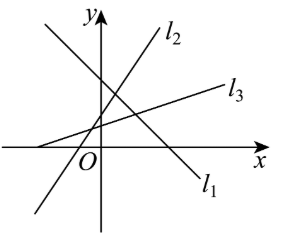
\includegraphics[width=0.15\textwidth]{chapters/linear-circle/images/直线与圆的基本概念/img-20250707161548.png}
    \end{figure}

    \begin{tasks}(4)
        \task $k_1<k_3<k_2$
        \task $k_3<k_2<k_1$
        \task $\alpha_1<\alpha_3<\alpha_2$
        \task $\alpha_3<\alpha_2<\alpha_1$
    \end{tasks}
\end{example}

\begin{definition}[一般式]
    已知 $A, B$ 不同时为 $0$，其标准方程为 $Ax+By+C=0$.

    一般式非常通用，可以直接表示任何直线（不需要讨论斜率不存在的情况）。
\end{definition}

\v{2em}

\begin{definition}[点斜式]
    已知直线的斜率 $k$ 和直线上一点 $(x_0, y_0)$，则直线的方程为 $y - y_0 = k(x - x_0)$。
\end{definition}

\begin{warning}
    这将是高中阶段最重要的式子！请务必熟记。
\end{warning}

\begin{example}
    已知 $\triangle A B C$ 的三个顶点是 $A(1,4), B(5,7), C(7,-4)$
    \begin{itemize}
        \item （1）求 $B C$ 边上的中线的直线方程；
        \item （2）求 $B C$ 边上的高的直线方程
    \end{itemize}
\end{example}

\v{6em}

\begin{definition}[两点式]
    已知两点 $A(x_1, y_1)$ 和 $B(x_2, y_2)$，则直线 $AB$ 的方程为 $\frac{y-y_1}{y_2-y_1} = \frac{x-x_1}{x_2-x_1}$，其中 $x_2 \neq x_1$ 且 $y_2 \neq y_1$.
\end{definition}

\begin{example}
    用两点式来表达直线的方程：
    \begin{itemize}
        \item 已知点 $A(1,2)$ 和点 $B(3,4)$，求直线 $AB$ 的方程。
        \item 求经过两点 $A(2,m)$ 和 $B(n,3)$ 的直线方程。
    \end{itemize}
\end{example}

\v{2em}

\begin{definition}[截距式]
    已知 $x, y$ 轴上的截距 $a, b$ 且 $ab \neq 0$，其标准方程为 $\frac{x}{a} + \frac{y}{b} = 1$。

    其中直线既不能垂直于 $x$ 轴，也不能垂直于 $y$ 轴，且不过原点。
\end{definition}

\begin{example}
    求过点 $(4,3)$ 且在两坐标轴上截距相等的直线 $l$ 的方程。
\end{example}

\begin{solution}
    设直线在 $x$ 轴、 $y$ 轴上的截距分别为 $a, b$ ．

    （1）当 $a \neq 0, b \neq 0$ 时，设 $l$ 的方程为 $\frac{x}{a}+\frac{y}{b}=1$. \\
    $\because$ 点 $(4,-3)$ 在直线上，$\therefore \frac{4}{a}-\frac{3}{b}=1$ ，
    若 $a=b$ ，则 $a=b=1$ ，直线方程为 $x+y-1=0$ ．

    （2）当 $a=b=0$ 时，直线过原点，且过点 $(4,-3)$. \\
    $\therefore$ 直线的方程为 $3 x+4 y=0$ ．
    综上知，所求直线方程为 $x+y-1=0$ 或 $3 x+4 y=0$ ．
\end{solution}

\begin{warning}
    在坐标轴上截距相等，有可能都为 $0$，即一条过原点的直线也会满足这个条件。
\end{warning}

\subsection{多种直线表达式的回顾}
\begin{center}
    \begin{tabular}{|c|c|c|c|}
        \hline
        \textbf{名称} & \textbf{已知条件}                                             & \textbf{标准方程}                                   & \textbf{使用范围}            \\
        \hline
        点斜式         & 斜率 $k$, 直线上一点 $(x_0,y_0)$                                 & $y-y_0 = k(x-x_0)$                              & $k$ 存在                   \\
        \hline
        斜截式         & 斜率 $k$, $y$ 轴截距 $b$                                       & $y=kx+b$                                        & $k$ 存在                   \\
        \hline
        两点式         & $(x_1, y_1)$, $(x_2, y_2)$ ($x_1 \neq x_2, y_1 \neq y_2$) & $\frac{y-y_1}{y_2-y_1} = \frac{x-x_1}{x_2-x_1}$ & 直线不能垂直于 $x$、$y$ 轴        \\
        \hline
        截距式         & $x,y$ 轴上的截距 $a,b$ ($ab \neq 0$)                           & $\frac{x}{a} + \frac{y}{b} = 1$                 & 直线不能垂直于 $x$、$y$ 轴, 且不过原点 \\
        \hline
        一般式         & $A, B$ 不同时为 $0$                                           & $Ax+By+C=0$                                     & 通用                       \\
        \hline
    \end{tabular}
\end{center}

\begin{problem}
求下列直线方程：

（1）若直线 $l$ 经过点 $A(2,-1), B(2,7)$ ，则直线 $l$ 的方程为 \underline{$\qquad$}.

（2）若点 $P(3, m)$ 在过点 $A(2,-1), B(-3,4)$ 的直线上，则 $m=$ \underline{$\qquad$}.
\end{problem}

\v{4em}

\begin{example}
    已知直线 $l: 3x + 4y - 12 = 0$ 和点 $A(1,2)$，求过点 $A$ 且与 $l$ 平行的直线方程，以及过点 $A$ 且与 $l$ 垂直的直线方程。
\end{example}

\v{4em}

\begin{example}
    求过点 $(1, -2)$ 且斜率为 $3$ 的直线的方程。
\end{example}
\begin{solution}
    使用点斜式方程 $y - y_0 = k(x - x_0)$。
    代入点 $(1, -2)$ 和斜率 $k=3$：
    $y - (-2) = 3(x - 1)$
    $y + 2 = 3x - 3$
    $y = 3x - 5$
\end{solution}

\begin{problem}
\begin{enumerate}
    \item 求过点 $(-2, 5)$ 且与直线 $2x - y + 1 = 0$ 平行的直线的方程。
          \vspace{6em}
    \item 已知直线 $L$ 的斜率为 $-\frac{1}{2}$，且在 $y$ 轴上的截距为 $4$，求直线 $L$ 的方程。
          \vspace{6em}
    \item 若直线 $ax + 2y - 1 = 0$ 与直线 $3x + y + 2 = 0$ 垂直，求实数 $a$ 的值。
\end{enumerate}
\end{problem}

\subsection*{2. 椭圆的离心率或离心率的取值范围}
\begin{theorem}
    椭圆的标准方程为 $\frac{x^2}{a^2} + \frac{y^2}{b^2} = 1$ (焦点在 $x$ 轴上，$a>b>0$) 或 $\frac{y^2}{a^2} + \frac{x^2}{b^2} = 1$ (焦点在 $y$ 轴上，$a>b>0$)。
    离心率 $e = \frac{c}{a}$，其中 $c^2 = a^2 - b^2$。
    离心率的取值范围是 $0 < e < 1$。
    当 $e \to 0$ 时，椭圆趋近于圆；当 $e \to 1$ 时，椭圆趋近于线段。
\end{theorem}

\begin{problem}
\begin{enumerate}
    \item 若椭圆的焦距为 $6$，长轴长为 $10$，求其离心率。
          \vspace{6em}
    \item 已知椭圆的短轴长为 $6$，离心率为 $\frac{\sqrt{3}}{2}$，求椭圆的长轴长。
          \vspace{6em}
    \item 设椭圆 $\frac{x^2}{m^2} + \frac{y^2}{4} = 1$ 的离心率为 $\frac{1}{2}$，求 $m$ 的值。
\end{enumerate}
\end{problem}

\subsection*{3. 简单复合函数的导数；某点处的导数值}

\begin{theorem}
    若 $y = f(u)$ 且 $u = g(x)$，则复合函数 $y = f(g(x))$ 的导数为 $\frac{dy}{dx} = \frac{dy}{du} \cdot \frac{du}{dx}$ (链式法则)。
    即 $y' = f'(g(x)) \cdot g'(x)$。
\end{theorem}

\begin{example}
    求函数 $y = (2x + 1)^3$ 的导数，并计算其在 $x=1$ 处的导数值。
\end{example}
\begin{solution}
    设 $u = 2x+1$，则 $y = u^3$。
    因为 $u = 2x+1$，所以 $u'_x = 2$。
    又因为 $y = u^3$，所以 $y'_u = 3u^2$。
    根据复合函数求导法则 $y'_x = y'_u \cdot u'_x = 3u^2 \cdot 2 = 6u^2$。
    将 $u = 2x+1$ 代回，得到 $y'_x = 6(2x+1)^2$。
    当 $x=1$ 时，$y'_x|_{x=1} = 6(2 \cdot 1 + 1)^2 = 6(3)^2 = 6 \cdot 9 = 54$。
\end{solution}

\begin{problem}
\begin{enumerate}
    \item 求函数 $f(x) = \sin(3x - \frac{\pi}{4})$ 的导数。
          \vspace{6em}
    \item 求函数 $y = e^{x^2}$ 在 $x=0$ 处的导数值。
          \vspace{6em}
    \item 已知函数 $g(x) = \sqrt{x^2 + 5}$，求 $g'(2)$。
\end{enumerate}
\vspace{6em}
\end{problem}

\subsection*{4. 根据方程表示双曲线求参数的范围}
\begin{theorem}
    双曲线的标准方程有两种形式：
    1.  焦点在 $x$ 轴上：$\frac{x^2}{a^2} - \frac{y^2}{b^2} = 1$ ($a>0, b>0$)。
    2.  焦点在 $y$ 轴上：$\frac{y^2}{a^2} - \frac{x^2}{b^2} = 1$ ($a>0, b>0$)。
    无论哪种形式，双曲线的定义都要求 $a^2$ 和 $b^2$ 为正数。
    关键在于，标准方程中，位于正号下方的分母是 $a^2$，它不一定是较大的那个分母。
\end{theorem}

\begin{example}
    若方程 $\frac{x^2}{k-2} - \frac{y^2}{3-k} = 1$ 表示双曲线，求实数 $k$ 的取值范围。
\end{example}
\begin{solution}
    要使方程表示双曲线，必须满足分母均为正数，即 $k-2 > 0$ 且 $3-k > 0$。
    由 $k-2 > 0$ 得到 $k > 2$。
    由 $3-k > 0$ 得到 $k < 3$。
    综合以上两点，实数 $k$ 的取值范围是 $2 < k < 3$。
\end{solution}

\begin{problem}
\begin{enumerate}
    \item 若方程 $\frac{y^2}{m+1} - \frac{x^2}{4-m} = 1$ 表示双曲线，求实数 $m$ 的取值范围。
          \vspace{6em}
    \item 判断方程 $3x^2 - 4y^2 = 12$ 是否表示双曲线，如果是，写出其标准方程。
          \vspace{6em}
    \item 已知方程 $x^2 - ky^2 = 1$ 表示双曲线，求实数 $k$ 的取值范围。
\end{enumerate}
\end{problem}
\begin{tips}
    双曲线的判断条件是 $x^2$ 和 $y^2$ 项的系数符号相反。对于标准方程，必须是正数减正数的形式。
\end{tips}
\begin{warning}
    与椭圆不同，双曲线的 $a$ 和 $b$ 的大小关系不确定，但 $a^2$ 始终是正号下方那个项的分母。
\end{warning}

\subsection*{5. 求指定项的系数}
\begin{theorem}
    对于二项式定理展开式 $(a+b)^n = \sum_{k=0}^{n} \binom{n}{k} a^{n-k} b^k$，其中 $\binom{n}{k} = \frac{n!}{k!(n-k)!}$ 是二项式系数。
    通项公式为 $T_{k+1} = \binom{n}{k} a^{n-k} b^k$。
    要求指定项的系数，通常是根据通项公式，令某变量的指数满足要求，然后解出 $k$ 的值。
\end{theorem}

\begin{example}
    求 $(2x - \frac{1}{x})^6$ 展开式中常数项。
\end{example}
\begin{solution}
    通项公式为 $T_{k+1} = \binom{6}{k} (2x)^{6-k} (-\frac{1}{x})^k = \binom{6}{k} 2^{6-k} x^{6-k} (-1)^k x^{-k}$。
    $= \binom{6}{k} 2^{6-k} (-1)^k x^{6-k-k} = \binom{6}{k} 2^{6-k} (-1)^k x^{6-2k}$。
    要使 $x$ 的指数为 $0$ (常数项)，令 $6-2k = 0$，解得 $k=3$。
    将 $k=3$ 代入系数部分：
    $\binom{6}{3} 2^{6-3} (-1)^3 = \frac{6!}{3!3!} \cdot 2^3 \cdot (-1) = \frac{6 \cdot 5 \cdot 4}{3 \cdot 2 \cdot 1} \cdot 8 \cdot (-1) = 20 \cdot 8 \cdot (-1) = -160$。
    常数项为 $-160$。
\end{solution}

\begin{problem}
\begin{enumerate}
    \item 求 $(x^2 - \frac{1}{x})^8$ 展开式中 $x^4$ 的系数。
          \vspace{6em}
    \item 求 $(\sqrt{x} + \frac{2}{x})^9$ 展开式中常数项。
          \vspace{6em}
    \item 求 $(1 + x)^n$ 展开式中 $x^2$ 的系数是 $15$，求 $n$ 的值。
\end{enumerate}
\end{problem}

\subsection*{6. 瞬时变化率的概念及解析；某点处的导数值}

\begin{theorem}
    瞬时变化率是指函数在某一点处的变化速度，它在数值上等于该点处的导数。
    若函数为 $y=f(x)$，则其在 $x_0$ 处的瞬时变化率为 $f'(x_0) = \lim_{\Delta x \to 0} \frac{f(x_0 + \Delta x) - f(x_0)}{\Delta x}$。
    它反映了函数值随自变量变化而变化的快慢程度。
\end{theorem}

\begin{example}
    求函数 $f(x) = x^2 + 3x$ 在 $x=2$ 处的瞬时变化率。
\end{example}
\begin{solution}
    首先求函数的导数 $f'(x)$。
    $f'(x) = \frac{d}{dx}(x^2 + 3x) = 2x + 3$。
    然后将 $x=2$ 代入导数表达式：
    $f'(2) = 2(2) + 3 = 4 + 3 = 7$。
    因此，函数 $f(x) = x^2 + 3x$ 在 $x=2$ 处的瞬时变化率为 $7$。
\end{solution}

\begin{problem}
\begin{enumerate}
    \item 求函数 $f(x) = \frac{1}{x}$ 在 $x=1$ 处的瞬时变化率。
          \vspace{6em}
    \item 某物体运动的位移 $s$ (单位：米) 与时间 $t$ (单位：秒) 的关系为 $s(t) = 5t^2 - 2t + 1$，求物体在 $t=2$ 秒时的瞬时速度。
          \vspace{6em}
    \item 已知函数 $h(x) = x^3 - 2x^2 + x - 1$，求当 $x=1$ 时函数值的瞬时变化率。
\end{enumerate}
\end{problem}
\begin{tips}
    瞬时变化率就是导数的几何意义，表示曲线在某点的切线斜率。
\end{tips}
\begin{warning}
    区分平均变化率（割线斜率）和瞬时变化率（切线斜率）。
\end{warning}

\subsection*{7. 抛物线的焦半径公式；根据抛物线上的点求标准方程}
\begin{theorem}
    对于抛物线 $y^2 = 2px$ ($p>0$)，焦点为 $F(\frac{p}{2}, 0)$，准线为 $x = -\frac{p}{2}$。
    任意一点 $M(x_0, y_0)$ 到焦点的距离（焦半径）为 $|MF| = x_0 + \frac{p}{2}$。
    对于抛物线 $x^2 = 2py$ ($p>0$)，焦点为 $F(0, \frac{p}{2})$，准线为 $y = -\frac{p}{2}$。
    任意一点 $M(x_0, y_0)$ 到焦点的距离（焦半径）为 $|MF| = y_0 + \frac{p}{2}$。
    根据抛物线上一点和其定义（到焦点和准线距离相等）或代入法，可以求其标准方程。
\end{theorem}

\begin{example}
    已知抛物线 $y^2 = 4x$，点 $P(4, y_0)$ 在抛物线上，求点 $P$ 到焦点的距离。
\end{example}
\begin{solution}
    抛物线方程 $y^2 = 4x$ 可知 $2p=4$，所以 $p=2$。
    焦点为 $F(\frac{p}{2}, 0) = F(1, 0)$。
    点 $P(4, y_0)$ 的横坐标为 $x_0 = 4$。
    根据焦半径公式 $|PF| = x_0 + \frac{p}{2} = 4 + \frac{2}{2} = 4 + 1 = 5$。
    点 $P$ 到焦点的距离为 $5$。
\end{solution}

\begin{problem}
\begin{enumerate}
    \item 已知抛物线 $x^2 = 8y$，求点 $Q(x_0, 2)$ 到焦点的距离。
          \vspace{6em}
    \item 若抛物线过点 $(2, 4)$，且顶点在原点，焦点在 $y$ 轴上，求该抛物线的标准方程。
          \vspace{6em}
    \item 设点 $A(3, m)$ 在抛物线 $y^2 = 6x$ 上，求点 $A$ 到抛物线准线的距离。
\end{enumerate}
\end{problem}
\begin{tips}
    抛物线的焦半径公式是利用定义推导出来的，记住它的形式可以简化计算。
\end{tips}
\begin{warning}
    确定抛物线焦点的位置和开口方向，才能正确选择焦半径公式。
\end{warning}

\subsection*{8. 总体百分位的估计}
\begin{theorem}
    百分位是将一组数据从小到大排列后，处于特定百分比位置的数据值。
    对于离散数据，第 $P$ 百分位的估计通常通过以下步骤进行：
    \begin{enumerate}
        \item 将数据按升序排列。
        \item 计算位置指数 $L = \frac{P}{100} \times n$，其中 $P$ 是百分位数 (如 $25$ 代表 $25\%$)，$n$ 是数据总数。
        \item 如果 $L$ 是整数，则第 $P$ 百分位是排序后的第 $L$ 个数据和第 $L+1$ 个数据的平均值。
        \item 如果 $L$ 不是整数，则将 $L$ 向上取整到下一个整数，第 $P$ 百分位是排序后的该位置的数据。
    \end{enumerate}
    对于连续数据或大样本数据，百分位的估计通常通过累计频率分布图或插值法进行。
\end{theorem}

\begin{example}
    某班级 $10$ 名学生的数学成绩 (从小到大排列) 如下：
    $60, 65, 70, 75, 80, 85, 90, 92, 95, 98$。
    估计该班学生数学成绩的第 $75$ 百分位。
\end{example}
\begin{solution}
    数据总数 $n=10$。
    要估计第 $75$ 百分位，即 $P=75$。
    计算位置指数 $L = \frac{75}{100} \times 10 = 7.5$。
    由于 $L$ 不是整数，向上取整为 $8$。
    因此，第 $75$ 百分位是排序后的第 $8$ 个数据。
    从排序后的数据中，第 $8$ 个数据是 $92$。
    所以，该班学生数学成绩的第 $75$ 百分位是 $92$ 分。
\end{solution}

\begin{problem}
\begin{enumerate}
    \item 某公司 $15$ 名员工的月薪 (单位：元) 如下：
          $$4000, 4200, 4500, 4800, 5000, 5200, 5500, 5800, 6000, 6200, 6500, 6800, 7000, 7500, 8000$$
          估计该员工月薪的第 $25$ 百分位。
          \vspace{6em}
    \item 一组数据的第 $50$ 百分位是 $85$，这意味着什么？
          \vspace{6em}
    \item 某次考试成绩的第 $80$ 百分位是 $90$ 分，若参加考试的学生有 $200$ 人，估计有多少学生的成绩低于或等于 $90$ 分？
\end{enumerate}
\end{problem}

\subsection*{9. 二项展开式各项的系数和}

\begin{theorem}
    对于二项式 $(a+b)^n$ 的展开式 $C_n^0 a^n + C_n^1 a^{n-1}b + \cdots + C_n^k a^{n-k}b^k + \cdots + C_n^n b^n$。
    其所有项的系数之和为：令 $a=1, b=1$，则展开式的值为 $(1+1)^n = 2^n$。
    若要求某个特定项的系数和，例如只包含 $x$ 的各项系数和，则将其他变量设为 $1$。
\end{theorem}

\begin{example}
    求 $(2x - y)^5$ 展开式中所有项的系数和。
\end{example}
\begin{solution}
    令 $x=1, y=1$，代入二项式 $(2x - y)^5$。
    则系数和为 $(2 \cdot 1 - 1)^5 = (2 - 1)^5 = 1^5 = 1$。
\end{solution}

\begin{problem}
\begin{enumerate}
    \item 求 $(x + 3y)^4$ 展开式中所有项的系数和。
          \vspace{6em}
    \item 求 $(2x^2 - x + 1)^3$ 展开式中所有项的系数和。
          \vspace{6em}
    \item 若 $(ax - 1)^6$ 展开式中所有项的系数和为 $64$，求实数 $a$ 的值。
\end{enumerate}
\end{problem}
\begin{tips}
    所有项的系数和的快速计算方法是将展开式中的所有变量替换为 $1$。
\end{tips}
\begin{warning}
    如果要求的是特定项的系数（而不是系数和），则需要使用通项公式。
\end{warning}

\subsection*{10. 计算典型问题的概率；独立事件的乘法公式}

\begin{theorem}
    $$\text{概率的基本公式：} P(A) = \frac{\text{事件A发生的有利结果数}}{\text{所有可能结果总数}}$$

    独立事件的乘法公式： 若事件 $A$ 和事件 $B$ 是相互独立的，则它们同时发生的概率为 $P(A \cap B) = P(A)P(B)$。

    推广到多个独立事件：如果 $A_1, A_2, \ldots, A_n$ 是相互独立的，则：
    $$P(A_1 \cap A_2 \cap \cdots \cap A_n) = P(A_1)P(A_2)\cdots P(A_n)$$
\end{theorem}

\begin{example}
    一个袋中有 $5$ 个红球和 $3$ 个白球，每次随机取出一个球，取出后放回。连续取两次，求两次都取到红球的概率。
\end{example}
\begin{solution}
    总球数 $= 5+3 = 8$ 个。
    设事件 $A$ 为第一次取到红球，事件 $B$ 为第二次取到红球。
    由于是放回抽样，所以两次抽取是相互独立的。
    $P(A) = \frac{5}{8}$。
    $P(B) = \frac{5}{8}$。
    两次都取到红球的概率为 $P(A \cap B) = P(A)P(B) = \frac{5}{8} \cdot \frac{5}{8} = \frac{25}{64}$。
\end{solution}

\begin{problem}
\begin{enumerate}
    \item 小明射击的命中率为 $0.8$，小红射击的命中率为 $0.7$，两人独立射击同一目标一次，求两人都命中的概率。
          \vspace{6em}
    \item 抛掷一枚均匀的硬币两次，求第一次正面朝上且第二次反面朝上的概率。
          \vspace{6em}
    \item 某产品生产线有甲、乙两道工序，甲工序的合格率为 $0.9$，乙工序的合格率为 $0.85$，两道工序相互独立。求该产品最终合格的概率。
\end{enumerate}
\end{problem}

\subsection*{11. 判断命题的充分必要条件；互斥事件与对立事件关系的辨析}
\begin{theorem}
    \begin{itemize}
        \item 充分条件：如果 $P$ 成立，则 $Q$ 必然成立，记作 $P \Rightarrow Q$。
        \item 必要条件：如果 $Q$ 成立，则 $P$ 必然成立，记作 $Q \Leftarrow P$。
        \item 充要条件：如果 $P$ 成立当且仅当 $Q$ 成立，记作 $P \Leftrightarrow Q$。
        \item 互斥事件：两个事件不能同时发生，记作 $A \cap B = \emptyset$。如果 $A, B$ 互斥，则 $P(A \cup B) = P(A) + P(B)$。
        \item 对立事件：如果 $A \cap B = \emptyset$
              且 $A \cup B = S$ (样本空间)，则 $A$ 和 $B$ 互为对立事件。对立事件一定是互斥事件，且 $P(A) + P(B) = 1$。
    \end{itemize}
\end{theorem}

\begin{example}
    判断：“$a>0$”是“$a^2>0$”的什么条件？
\end{example}
\begin{solution}
    1.  如果 $a>0$，则 $a^2>0$ 成立，所以 $a>0 \Rightarrow a^2>0$。因此，“$a>0$”是“$a^2>0$”的充分条件。

    2.  如果 $a^2>0$，则 $a \ne 0$。此时 $a$ 可以是 $a>0$ 或 $a<0$。例如，$a=-2$ 时 $a^2=4>0$，但 $a>0$ 不成立。所以 $a^2>0 \not\Rightarrow a>0$。因此，“$a^2>0$”不是“$a>0$”的充分条件，即“$a>0$”不是“$a^2>0$”的必要条件。

    综上所述，“$a>0$”是“$a^2>0$”的**充分不必要条件**。
\end{solution}

\begin{problem}
\begin{enumerate}
    \item 判断：“$x=1$”是“$x^2-3x+2=0$”的什么条件？
          \vspace{6em}
    \item 设 $A$ 和 $B$ 是样本空间 $S$ 中的两个事件。下列说法正确的是：
          \begin{itemize}
              \item A. 如果 $A, B$ 互斥，则 $P(A)+P(B)=1$。
              \item B. 如果 $A, B$ 对立，则 $A, B$ 互斥。
              \item C. 如果 $P(A)=0.5, P(B)=0.5$，则 $A, B$ 对立。
              \item D. 互斥事件一定是独立事件。
          \end{itemize}
          \vspace{6em}
\end{enumerate}

\end{problem}

\subsection*{12. 元素 (位置) 有限的排列问题；不相邻排列问题}

\begin{theorem}
    排列数公式：从 $n$ 个不同元素中取出 $m$ 个元素，按照一定的顺序排成一列，叫做从 $n$ 个不同元素中取出 $m$ 个元素的排列。排列数 $A_n^m = \frac{n!}{(n-m)!}$。

    不相邻排列问题 (插空法)：在排列中，若要求某些元素互不相邻，通常采用“先排好不相邻的元素，再将要不相邻的元素插入已排好的元素之间的空隙”的方法。

    步骤：
    \begin{itemize}
        \item 先排列允许相邻的元素。
        \item 找出这些元素产生的空隙。
        \item 将互不相邻的元素插入这些空隙。
    \end{itemize}
\end{theorem}

\begin{example}
    有 $5$ 个人排成一排，其中甲、乙两人不能相邻，有多少种不同的排法？
\end{example}
\begin{solution}
    方法一：插空法
    1.  先排列除了甲、乙以外的 $3$ 个人 (丙、丁、戊)，有 $A_3^3 = 3! = 6$ 种排法。

    2.  这 $3$ 个人排好后，会产生 $4$ 个空隙 (包括两端)：$\_ P_1 \_ P_2 \_ P_3 \_$。

    3.  将甲、乙插入这 $4$ 个空隙中的任意两个，有 $A_4^2 = 4 \times 3 = 12$ 种方法。
    总排法数 $= A_3^3 \times A_4^2 = 6 \times 12 = 72$ 种。

    方法二：间接法 (排除法)
    1.  总排法数：$5$ 个人全排列有 $A_5^5 = 5! = 120$ 种。

    2.  甲、乙相邻的排法数：将甲、乙捆绑成一个整体，看作 $1$ 个人。

    则共有 $4$ 个“人”进行全排列，有 $A_4^4 = 4! = 24$ 种排法。

    甲、乙自身可以交换位置，有 $2! = 2$ 种排法。

    所以甲、乙相邻的排法数 $= 24 \times 2 = 48$ 种。

    3.  甲、乙不能相邻的排法数 = 总排法数 - 甲、乙相邻的排法数 $= 120 - 48 = 72$ 种。
\end{solution}

\begin{problem}
\begin{enumerate}
    \item 从 $7$ 名学生中选出 $3$ 人排成一列，有多少种不同的排法？
          \vspace{6em}
    \item 某班有 $3$ 名男生和 $2$ 名女生，排成一排。如果 $2$ 名女生不能相邻，有多少种不同的排法？
          \vspace{6em}
    \item 用 $0, 1, 2, 3, 4$ 这五个数字组成没有重复数字的五位数，其中偶数有多少个？
\end{enumerate}
\end{problem}

\subsection*{13. 函数与导数图像关系；拐点；图象与极值的关系；求切线的斜率 (倾斜角)}

\begin{theorem}
    \begin{itemize}
        \item \textbf{函数与导数图像关系：}
              \begin{itemize}
                  \item 当 $f'(x) > 0$ 时，$f(x)$ 单调递增。
                  \item 当 $f'(x) < 0$ 时，$f(x)$ 单调递减。
                  \item 当 $f'(x) = 0$ 时，可能存在极值点（驻点）。
              \end{itemize}

        \item \textbf{极值点：} 函数在某点 $x_0$ 处取得极值，如果 $f'(x_0)=0$，并且 $f'(x)$ 在 $x_0$ 附近改变符号。
              \begin{itemize}
                  \item 从正变负：极大值点。
                  \item 从负变正：极小值点。
              \end{itemize}

        \item \textbf{切线的斜率 (倾斜角)：} 曲线 $y=f(x)$ 在点 $(x_0, y_0)$ 处的切线斜率等于该点处的导数 $f'(x_0)$。切线的倾斜角 $\theta$ 满足 $\tan \theta = f'(x_0)$，其中 $0 \le \theta < \pi$。
    \end{itemize}
\end{theorem}

\begin{example}
    求函数 $f(x) = x^3 - 3x^2 + 1$ 在点 $(1, -1)$ 处的切线斜率和倾斜角。
\end{example}
\begin{solution}
    首先求函数的导数 $f'(x)$：
    $f'(x) = 3x^2 - 6x$。
    在点 $(1, -1)$ 处，切线斜率 $k = f'(1) = 3(1)^2 - 6(1) = 3 - 6 = -3$。
    切线的倾斜角 $\theta$ 满足 $\tan \theta = -3$。
    由于 $\tan \theta < 0$，且 $0 \le \theta < \pi$，所以倾斜角 $\theta$ 是钝角。
    $\theta = \arctan(-3) + \pi$ (如果计算器给出的是负角，需要加 $\pi$)。
\end{solution}

\begin{problem}
\begin{enumerate}
    \item 求函数 $y = x^2 - 4x + 3$ 的单调区间和极值点。
          \vspace{6em}
    \item 已知函数 $f(x) = ax^3 + bx^2 + c$ 在 $x=1$ 处有极小值 $-2$，且其导数在 $x=0$ 处为 $0$，求 $a, b, c$ 的值。
          \vspace{6em}
    \item 求函数 $f(x) = x \ln x$ 在 $x=e$ 处的切线方程。
\end{enumerate}
\end{problem}
\begin{tips}
    通过导数符号的变化来判断函数的增减性，通过二阶导数符号的变化来判断函数的凹凸性。
\end{tips}
\begin{warning}
    求极值点时，仅仅 $f'(x)=0$ 不足以说明是极值点，还需要检查导数符号是否改变。
\end{warning}

\subsection*{14. 过圆上一点的圆的切线方程；求切线斜率 (倾斜角)}
\begin{theorem}
    过圆上一点的切线方程：

    设圆的方程为 $(x-a)^2 + (y-b)^2 = R^2$，圆上一点为 $(x_0, y_0)$。
    则过点 $(x_0, y_0)$ 的切线方程为 $(x_0-a)(x-a) + (y_0-b)(y-b) = R^2$。

    特别地，当圆心在原点时，圆的方程为 $x^2 + y^2 = R^2$，切线方程为 $x_0x + y_0y = R^2$。
\end{theorem}

\begin{example}
    求圆 $x^2 + y^2 = 5$ 在点 $(1, 2)$ 处的切线方程。
\end{example}
\begin{solution}
    方法一：使用公式
    圆心在原点 $(0,0)$，半径 $R^2=5$。切点 $(x_0, y_0) = (1, 2)$。
    切线方程为 $x_0x + y_0y = R^2$。
    代入得到 $1 \cdot x + 2 \cdot y = 5$，即 $x + 2y = 5$。

    方法二：利用垂直关系
    圆心为 $O(0,0)$，切点为 $P(1,2)$。
    半径 $OP$ 的斜率为 $k_{OP} = \frac{2-0}{1-0} = 2$。
    由于切线垂直于半径，所以切线斜率 $k_{切线} = -\frac{1}{k_{OP}} = -\frac{1}{2}$。
    切线过点 $(1,2)$，使用点斜式方程：$y - 2 = -\frac{1}{2}(x - 1)$。
    $2(y - 2) = -(x - 1)$
    $2y - 4 = -x + 1$
    $x + 2y = 5$。
\end{solution}

\begin{problem}
\begin{enumerate}
    \item 求圆 $(x-2)^2 + (y+1)^2 = 10$ 在点 $(3, 2)$ 处的切线方程。
          \vspace{6em}
    \item 已知直线 $y = x + m$ 与圆 $x^2 + y^2 = 2$ 相切，求实数 $m$ 的值。
          \vspace{6em}
    \item 若圆 $C$ 的方程为 $x^2 + y^2 - 4x + 6y - 3 = 0$，求过圆上一点 $P(1, 0)$ 的切线方程。
\end{enumerate}
\end{problem}
\begin{tips}
    记住圆的切线公式可以快速解题。如果忘记公式，可以使用“切线垂直于半径”的几何性质。
\end{tips}
\begin{warning}
    过圆外一点作圆的切线，其方法与过圆上一点不同，通常需要用到点到直线的距离公式。
\end{warning}

\section*{三、解答题}

\subsection*{15. 利用导数求函数的单调区间 (不含参)；求已知函数的极值}
\begin{theorem}
    利用导数判断单调性：
    设函数 $f(x)$ 在区间 $(a,b)$ 内可导。

    \begin{itemize}
        \item     若 $f'(x) > 0$ 对任意 $x \in (a,b)$ 成立，则 $f(x)$ 在 $(a,b)$ 上单调递增。
        \item     若 $f'(x) < 0$ 对任意 $x \in (a,b)$ 成立，则 $f(x)$ 在 $(a,b)$ 上单调递减。
    \end{itemize}


    \begin{theorem}[利用导数求极值：]
    \end{theorem}
    \begin{enumerate}
        \item 求出导函数 $f'(x)$。
        \item 令 $f'(x)=0$，解出所有驻点。
        \item 检查这些驻点左右两侧 $f'(x)$ 的符号。如果符号改变，则为极值点。
    \end{enumerate}
\end{theorem}

\begin{example}
    求函数 $f(x) = x^3 - 6x^2 + 9x - 1$ 的单调区间和极值。
\end{example}
\begin{solution}
    1.  求导：$f'(x) = 3x^2 - 12x + 9$。

    2.  令 $f'(x) = 0$，即 $3x^2 - 12x + 9 = 0$，简化为 $x^2 - 4x + 3 = 0$。
    解得 $(x-1)(x-3) = 0$，所以驻点为 $x=1, x=3$。

    3.  分析 $f'(x)$ 的符号：
    * 当 $x < 1$ 时 (如 $x=0$)，$f'(0) = 9 > 0$，所以 $f(x)$ 单调递增。

    * 当 $1 < x < 3$ 时 (如 $x=2$)，$f'(2) = 3(4) - 12(2) + 9 = 12 - 24 + 9 = -3 < 0$，所以 $f(x)$ 单调递减。

    * 当 $x > 3$ 时 (如 $x=4$)，$f'(4) = 3(16) - 12(4) + 9 = 48 - 48 + 9 = 9 > 0$，所以 $f(x)$ 单调递增。

    4.  确定单调区间和极值：

    * 单调递增区间：$(-\infty, 1)$ 和 $(3, +\infty)$。

    * 单调递减区间：$(1, 3)$。

    * 在 $x=1$ 处，$f'(x)$ 从正变负，有极大值 $f(1) = 1^3 - 6(1)^2 + 9(1) - 1 = 1 - 6 + 9 - 1 = 3$。

    * 在 $x=3$ 处，$f'(x)$ 从负变正，有极小值 $f(3) = 3^3 - 6(3)^2 + 9(3) - 1 = 27 - 54 + 27 - 1 = -1$。
\end{solution}

\begin{problem}
\begin{enumerate}
    \item 求函数 $f(x) = \frac{1}{3}x^3 - x^2 - 3x + 1$ 的单调区间。
          \vspace{6em}
    \item 已知函数 $g(x) = x^4 - 2x^2$，求其所有极值点和极值。
          \vspace{6em}
    \item 函数 $h(x) = \frac{\ln x}{x}$ 在定义域内的单调区间。
\end{enumerate}
\end{problem}
\begin{tips}
    求单调区间和极值时，通常需要先求导，然后解方程和分析符号。
\end{tips}
\begin{warning}
    在写单调区间时，区间端点不要包含在开区间内；极值点只是 $x$ 的值，极值是 $y$ 的值。
\end{warning}

\subsection*{16. 利用事件的概率公式；独立事件的乘法公式；互斥事件的概率加法公式}

\begin{theorem}
    \begin{itemize}
        \item \textbf{概率的基本性质：} $0 \le P(A) \le 1$，$P(S) = 1$ (必然事件)，$P(\emptyset) = 0$ (不可能事件)。
        \item \textbf{互斥事件的加法公式：} 若事件 $A$ 和 $B$ 互斥，则 $P(A \cup B) = P(A) + P(B)$。
        \item \textbf{任意事件的加法公式：} $P(A \cup B) = P(A) + P(B) - P(A \cap B)$。
        \item \textbf{独立事件的乘法公式：} 若事件 $A$ 和 $B$ 相互独立，则 $P(A \cap B) = P(A)P(B)$。
        \item \textbf{对立事件的概率：} $P(A) + P(\bar{A}) = 1$，其中 $\bar{A}$ 是事件 $A$ 的对立事件。
    \end{itemize}
\end{theorem}

\begin{example}
    甲、乙两人各射击一次，甲命中目标的概率为 $0.6$，乙命中目标的概率为 $0.7$。假设两人射击相互独立，求：

    (1) 两人都命中的概率；

    (2) 至少一人命中的概率。
\end{example}

\begin{solution}
    设事件 $A$ 为甲命中目标，事件 $B$ 为乙命中目标。
    已知 $P(A) = 0.6$， $P(B) = 0.7$。

    由于两人射击相互独立，则 $P(\bar{A}) = 1 - 0.6 = 0.4$， $P(\bar{B}) = 1 - 0.7 = 0.3$。

    (1) 两人都命中的概率为 $P(A \cap B)$。
    由于 $A, B$ 独立，所以 $P(A \cap B) = P(A)P(B) = 0.6 \times 0.7 = 0.42$。

    (2) 至少一人命中的概率为 $P(A \cup B)$。

    方法一：使用加法公式 $P(A \cup B) = P(A) + P(B) - P(A \cap B) = 0.6 + 0.7 - 0.42 = 1.3 - 0.42 = 0.88$。

    方法二：使用对立事件，即“至少一人命中”的对立事件是“两人都未命中”。

    $P(\text{两人都未命中}) = P(\bar{A} \cap \bar{B})$。

    由于 $\bar{A}, \bar{B}$ 也相互独立，所以 $P(\bar{A} \cap \bar{B}) = P(\bar{A})P(\bar{B}) = 0.4 \times 0.3 = 0.12$。

    所以，$P(A \cup B) = 1 - P(\bar{A} \cap \bar{B}) = 1 - 0.12 = 0.88$。
\end{solution}

\begin{problem}
\begin{enumerate}
    \item 某次考试，甲同学通过的概率是 $0.7$，乙同学通过的概率是 $0.8$，假设他们通过与否相互独立。求甲未通过但乙通过的概率。
          \vspace{6em}
    \item 在一个盒子中有 $3$ 个红球和 $2$ 个白球。从中随机抽取一个球，然后放回，再抽取一个球。求两次抽取的球颜色相同的概率。
          \vspace{6em}
    \item 袋中有 $5$ 个大小相同的小球，其中 $3$ 个白球，$2$ 个黑球。从中一次摸出 $2$ 个球，求摸出的 $2$ 个球颜色相同的概率。
\end{enumerate}
\end{problem}
\begin{tips}
    在解决概率问题时，首先明确事件之间的关系（独立、互斥、对立），然后选择合适的公式。
\end{tips}
\begin{warning}
    “互斥”与“独立”是完全不同的概念，不要混淆其公式应用。
\end{warning}

\subsection*{17. 由频率分布直方图计算频率、频率、样本容量、总体容量；由频率分布直方图估计中位数}

\begin{theorem}
    \textbf{频率分布直方图的性质：}

    1. 小长方形的面积表示该组的频率。频率 = $\text{组距} \times \text{频率/组距 (即高度)}$。

    2. 所有小长方形的面积之和为 $1$。

    3. 样本容量 = $\frac{\text{某组频数}}{\text{该组频率}}$。

    4. 总体容量通常无法直接从样本的频率分布直方图获得，但可以通过样本估计总体。

    \textbf{中位数估计：} 中位数是数据集中位于中间位置的数值。在频率分布直方图中，中位数位于累积频率达到 $0.5$ 的位置。

    估计方法：

    1. 找到使累积频率达到 $0.5$ 的那个矩形。

    2. 然后利用线性插值法计算中位数。
\end{theorem}

\begin{warning}
    频率分布直方图的横轴是分组，纵轴是频率/组距，而不是频率。
\end{warning}

\subsection*{18. 根据定义求抛物线的标准方程；直线与抛物线相交所得弦长；与抛物线焦点有关的几何性质}

\begin{theorem}
    \textbf{抛物线的定义:} 平面内与一个定点（焦点 $F$）和一条定直线（准线 $l$）距离相等的点的轨迹。

    \textbf{抛物线的标准方程:}
    \begin{enumerate}
        \item $y^2 = 2px$ ($p>0$)：焦点 $F(\frac{p}{2}, 0)$，准线 $x = -\frac{p}{2}$。
        \item $y^2 = -2px$ ($p>0$)：焦点 $F(-\frac{p}{2}, 0)$，准线 $x = \frac{p}{2}$。
        \item $x^2 = 2py$ ($p>0$)：焦点 $F(0, \frac{p}{2})$，准线 $y = -\frac{p}{2}$。
        \item $x^2 = -2py$ ($p>0$)：焦点 $F(0, -\frac{p}{2})$，准线 $y = \frac{p}{2}$。
    \end{enumerate}

    \textbf{弦长相关性质:}
    \begin{itemize}
        \item \textbf{弦长公式:} 直线 $y=kx+b$ 与抛物线 $y^2=2px$ 相交于 $A(x_1, y_1)$, $B(x_2, y_2)$，则弦长 $|AB| = \sqrt{1+k^2}|x_1-x_2|$ 或 $|AB| = \sqrt{1+\frac{1}{k^2}}|y_1-y_2|$。结合韦达定理计算。

        \item \textbf{焦点弦长:} 过焦点的弦叫做焦点弦。若抛物线为 $y^2=2px$，过焦点的弦两端点为 $A(x_1, y_1)$ 和 $B(x_2, y_2)$，则 $|AB| = x_1+x_2+p$。
        \item \textbf{焦点弦性质:} 焦点弦的两端点到准线的距离之和等于 $p$。
    \end{itemize}
\end{theorem}

\begin{example}
    已知抛物线 $y^2 = 4x$，直线 $y = x - 1$ 与该抛物线相交于 $A, B$ 两点，求弦 $AB$ 的长。
\end{example}

\begin{solution}
    将直线方程 $y = x - 1$ 代入抛物线方程 $y^2 = 4x$：

    设 $A(x_1, y_1), B(x_2, y_2)$。根据韦达定理，$x_1+x_2 = 6, x_1x_2 = 1$。

    所以 $|AB| = \sqrt{(x_1-x_2)^2 + (x_1-x_2)^2} = \sqrt{2(x_1-x_2)^2} = \sqrt{2}|x_1-x_2|$。

    又 $(x_1-x_2)^2 = (x_1+x_2)^2 - 4x_1x_2 = 6^2 - 4(1) = 36 - 4 = 32$。

    所以 $|AB| = \sqrt{2 \cdot 32} = \sqrt{64} = 8$。

    弦 $AB$ 的长为 $8$。
\end{solution}

\begin{problem}
\begin{enumerate}
    \item 已知抛物线的准线方程为 $y = -2$，顶点在原点，求抛物线的标准方程。
          \vspace{6em}
    \item 直线 $y = 2x + 3$ 与抛物线 $y^2 = 8x$ 相交于 $M, N$ 两点，求弦 $MN$ 的中点坐标。
          \vspace{6em}
    \item 设抛物线 $y^2 = 2px$ ( $p>0$ ) 的焦点为 $F$，过 $F$ 的直线与抛物线交于 $A, B$ 两点，若 $AF = 3FB$，求弦 $AB$ 的长。
\end{enumerate}
\end{problem}
\begin{tips}
    在求弦长时，将直线方程代入抛物线方程，得到关于一个变量的一元二次方程，然后利用韦达定理和弦长公式。
\end{tips}
\begin{warning}
    注意抛物线的开口方向和焦点、准线的位置，这会影响标准方程的形式和焦半径公式的选择。
\end{warning}
\subsection{利用导数求切线方程}

\begin{theorem}
    \textbf{求切线方程}:
    \begin{itemize}
        \item \textbf{在点 $P(x_0, y_0)$ 处的切线}: P在曲线上，斜率为 $k=f'(x_0)$，使用点斜式 $y-y_0 = k(x-x_0)$。
        \item \textbf{过点 $P(x_0, y_0)$ 的切线}: P不在曲线上，需设切点为 $(x_1, f(x_1))$，表示出切线方程，再将点P坐标代入求解。
    \end{itemize}
\end{theorem}
\begin{example}
    已知函数 $f(x) = x^{2}$.
    \begin{enumerate}
        \item[(1)] 求曲线 $y = f(x)$ 在点 $(2,f(2))$ 处的切线方程；
        \item[(2)] 求曲线 $y = f(x)$ 过点 $(2,0)$ 的切线方程.
    \end{enumerate}
\end{example}

\vspace{4em}

\begin{example}
    已知曲线 $y = f(x)$ 在 $x = 5$ 处的切线方程是 $y = - 2x + 8$，则 $f(5) + f'(5)$ 的值为（\quad）
    \begin{tasks}(4)
        \task $- 4$ \task $- 2$ \task $2$ \task $4$
    \end{tasks}
\end{example}

\vspace{4em}

\begin{example}
    已知函数 $f(x) = 1 - 2x - \sin x$，则曲线 $y = f(x)$ 在点 $(0,f(0))$ 处的切线方程为（\quad）
    \begin{tasks}(4)
        \task $3x + y - 1 = 0$
        \task $2x - y + 1 = 0$
        \task $3x - y + 1 = 0$
        \task $2x + y - 1 = 0$
    \end{tasks}
\end{example}

\vspace{4em}

\begin{example}
    曲线 $f(x)=\frac{\ln x}{x^2}+\frac{1}{x+1}$ 在 $(1, f(1))$ 处的切线方程为
    \underline{$\qquad$} ．
\end{example}

\vspace{4em}

\begin{example}
    曲线 $y=\left(x^2-2\right) \ln x+x$ 在点 $(1,1)$ 处的切线方程为 \underline{$\qquad$} ．
\end{example}

\vspace{4em}

\begin{example}
    已知 $f(x)$ 为偶函数，曲线 $y = f(x)$ 在点 $(2,f(2))$ 处的切线与直线 $4x - y - 3 = 0$ 垂直，设 $f(x)$ 的导函数为 $f'(x)$，则 $f'(-2) = \underline{\hspace{3cm}}$.
\end{example}

\vspace{4em}

\begin{example}
    已知直线 $y=a x$ 是曲线 $y=\ln x$ 的切线，则实数 $a=$ \underline{$\qquad$}.
\end{example}

\vspace{4em}

\begin{example}
    已知函数 $f(x)=a x^2-2$ 的图象在点 $(\sqrt{3}, f(\sqrt{3}))$ 处的切线的倾斜角为 $\frac{\pi}{3}$ ，则曲线 $y=f(x)$ 在点 $(1, f(1))$ 处的切线的方程为（\quad）
    \begin{tasks}(4)
        \task $2 x+2 y-5=0$
        \task $2 x-2 y-5=0$
        \task $2 x-2 y+1=0$
        \task $2 x+2 y+1=0$
    \end{tasks}
\end{example}

\begin{example}
    过点 $(1,6)$ 且与曲线 $y=2 x^3+4$ 相切的直线方程为（\quad）
    \begin{itemize}
        \item $6 x-y=0$
        \item $9 x-y-3=0$
        \item $6 x-y=0$ 或 $3 x-2 y+9=0$
        \item $9 x-y-3=0$ 或 $3 x+2 y-15=0$
    \end{itemize}
\end{example}

\v{4em}

\begin{example}
    已知函数 $f(x) = x^{3} + x - 16$.
    \begin{enumerate}
        \item[(1)] 直线 $l$ 为曲线 $y = f(x)$ 在点 $(2, -6)$ 处的切线，求直线 $l$ 的方程；
        \item[(2)] 求过原点且与曲线 $y = f(x)$ 相切的切线方程及切点坐标．
    \end{enumerate}
\end{example}

\v{4em}